% 2020 江苏卷 9：六角螺帽毛坯（正六棱柱挖去一个圆柱）
% 绘制依据：固定源 PDF 第 1115 面原图。正六棱柱竖放，顶面为压扁的正六边形（前后各一条水平边），
% 顶面中心为一个圆柱形内孔（椭圆口），孔壁用虚线画到底面的虚线椭圆；背面棱与底面的后侧棱为虚线。
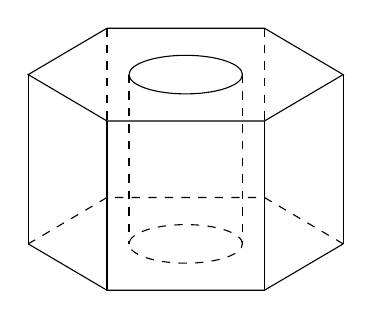
\begin{tikzpicture}[scale=1.0, font=\small]
  \def\r{2}
  \def\sq{0.34}
  \def\hh{2.15}
  % 顶面六顶点（角度 0,60,...,300），y 方向压缩为 \sq 倍
  \coordinate (P0) at ({\r*cos(0)},{\sq*\r*sin(0)});
  \coordinate (P1) at ({\r*cos(60)},{\sq*\r*sin(60)});
  \coordinate (P2) at ({\r*cos(120)},{\sq*\r*sin(120)});
  \coordinate (P3) at ({\r*cos(180)},{\sq*\r*sin(180)});
  \coordinate (P4) at ({\r*cos(240)},{\sq*\r*sin(240)});
  \coordinate (P5) at ({\r*cos(300)},{\sq*\r*sin(300)});
  % 底面六顶点：整体下移 \hh
  \coordinate (Q0) at ({\r*cos(0)},{\sq*\r*sin(0)-\hh});
  \coordinate (Q1) at ({\r*cos(60)},{\sq*\r*sin(60)-\hh});
  \coordinate (Q2) at ({\r*cos(120)},{\sq*\r*sin(120)-\hh});
  \coordinate (Q3) at ({\r*cos(180)},{\sq*\r*sin(180)-\hh});
  \coordinate (Q4) at ({\r*cos(240)},{\sq*\r*sin(240)-\hh});
  \coordinate (Q5) at ({\r*cos(300)},{\sq*\r*sin(300)-\hh});

  % 顶面轮廓（全可见，实线）
  \draw (P0) -- (P1) -- (P2) -- (P3) -- (P4) -- (P5) -- cycle;

  % 竖直棱：前面与左右两侧可见（实线），背面两条为虚线
  \draw (P0) -- (Q0);
  \draw (P3) -- (Q3);
  \draw (P4) -- (Q4);
  \draw (P5) -- (Q5);
  \draw[dashed] (P1) -- (Q1);
  \draw[dashed] (P2) -- (Q2);

  % 底面轮廓：前侧三条边可见（实线），后侧三条边被遮挡（虚线）
  \draw (Q3) -- (Q4) -- (Q5) -- (Q0);
  \draw[dashed] (Q0) -- (Q1) -- (Q2) -- (Q3);

  % 内孔：顶面椭圆口（实线），孔沿两条竖直线（虚线），底面椭圆（虚线）
  \draw (0,0) ellipse (0.72 and 0.245);
  \draw[dashed] (-0.72,0) -- (-0.72,-\hh);
  \draw[dashed] (0.72,0) -- (0.72,-\hh);
  \draw[dashed] (0,-\hh) ellipse (0.72 and 0.245);
\end{tikzpicture}
